\documentclass[hidelinks, 11pt, a4paper]{report}
\usepackage[margin=5cm]{geometry}
\usepackage{color, graphicx}
\usepackage[font=small]{caption}
\usepackage{diagbox}
\usepackage{amssymb}
\usepackage{fancyvrb}
\usepackage{subfiles}
\usepackage[pdfauthor=Phan Ngoc Lan - Nguyen Duy Manh, pdftitle={EvoComputing}, pdfsubject={WUSN} unicode, xetex,]{hyperref}
\usepackage{polyglossia}
\usepackage{ulem}
\usepackage{fontspec}
\usepackage{cite}
\usepackage{amsmath}

\setlength{\parindent}{0pt}
\setlength{\parskip}{6pt}
\graphicspath{ {images/} }
\setmainlanguage{vietnamese}
\pagenumbering{arabic}
\pagestyle{plain}

\newfontfamily\code{Courier New}
\newenvironment{codeb}{\code}{\par}

\begin{document}
\begin{titlepage}
    \begin{center}
        Đại học Bách Khoa Hà Nội\\
        Viện Công nghệ Thông tin và Truyền thông\\
        Bộ môn Khoa học máy tính\\
        
        \vspace{20pt}
        
        
\includegraphics[scale=0.08]{bklogo.jpg}
        
        \vspace{30pt}
        
        \Huge\textbf{Báo cáo cuối kì}
        
        \huge{Tính toán tiến hóa}
        
        \Large{Đề tài: Tối ưu hóa thời gian sống của mạng cảm biến không dây ngầm}\\
        
        \vspace{30pt}
        \textbf{Giảng viên hướng dẫn:}\\ PGS.TS Huỳnh Thị Thanh Bình
    
        \textbf{Sinh viên thực hiện:}\\
        Phan Ngọc Lân - 20142505\\
        Nguyến Duy Mạnh - 20142857
    \end{center}
\end{titlepage}

\newgeometry{left=4cm, right=4cm, bottom=4cm, top=3cm}
\setcounter{page}{1}

\tableofcontents

\chapter*{Phân công công việc}
\begin{table}[]
\centering
\begin{tabular}{|l|l|l|}
\hline
\textbf{Họ và tên} & \textbf{MSSV} & \textbf{Công việc} \\ \hline
Phan Ngọc Lân & 20142505 & Cài đặt thuật toán đề xuất. Viết báo cáo. \\ \hline
Nguyễn Duy Mạnh & 20142857 & Cài đặt các thuật toán heuristic. Làm slide thuyết trình. \\ \hline
\end{tabular}
\end{table}
\pagebreak

\chapter{Mở đầu}
\section{Giới thiệu bài toán}
Một mạng cảm biến không dây ngầm (Wireless Underground Sensor Networks - WUSNs) là mạng bao gồm các nút cảm biến được triển khai dưới mặt đất. Các cảm biến này thu thập và gửi dữ liệu thông qua các kết nối không dây.

Mạng cảm biến không dây ngầm có nhiều ứng dụng trong nông nghiệp, giám sát cơ sở hạ tầng, xác định vị trí đối tượng,...

Xem xét một mạng WUSN bao gồm các nút cảm biến ngầm (SNs), các nút chuyển tiếp (RNs) và trạm cơ sở (BS). Đây là mô hình mạng hai lớp: SNs chuyển dữ liệu đến RNs thông qua 1 hop.

Trong \cite{YuanWusn}, các tác giả đề xuất việc triển khai một số lượng giới hạn các nút chuyển tiếp để tối đa hóa tuổi thọ của mạng dưới các ràng buộc: cân bằng tải, topo mạng và mô hình thực tế.

Tuổi thọ mạng: khoảng thời gian từ lúc khởi tạo mạng cho đến lúc mạng bị tắt. Mạng bị tắt khi:
\begin{itemize}
    \item 1 nút hết năng lượng (N of N)
    \item $N − K + 1$ nút hết năng lượng (K of N)
\end{itemize}

\section{Mô hình}
\subsection{Mô hình truyền}
Mất mát đường truyền giữa mỗi cặp SN-RN được tính dựa trên các công thức sau:
\begin{align*}
    & T_{UG-AG} = T_{UG} + T_{AG} + T_R\\
    & T_{AG} = -147.6 + 10\eta\log(d_{ag}) + 20\log(f)\\
    & T_{UG} = 6.4 + 20\log(d_{ug}) + 20\log\beta + 8.69\alpha d_{ug}\\
    & T_R = 0
\end{align*}
trong đó $T_{UG}$ là mất mát đường truyền từ SN đến mặt đất, $T_{AG}$ là mất mát đường truyền từ mặt đất đến RN, và $T_R$ là mất mát khúc xạ.

\begin{center}
    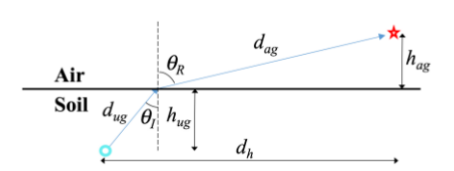
\includegraphics[scale=0.6]{transmission.png}
\end{center}

\subsection{Mô hình bài toán}
Ta mô hình hóa bài toán như sau:

\begin{itemize}
    \item {
        \textbf{Đầu vào:}
        \begin{itemize}
            \item $S = \{s_1, s_2, ..., s_N \}$: tập chứa tất cả nút cảm biến.
            \item $F = \{f_1, f_2, ..., f_M \}$: tập chứa tất cả các điểm có thể đặt relay.
            \item $Y$: số lượng relay phải đặt.
            \item $T = (t_{nm})_{NxM}$: mất mát đường truyền cho mỗi cặp SN-RN. Được tính dựa trên mô hình truyền.
        \end{itemize}
    }
    \item {
        \textbf{Đầu ra:}
        \begin{itemize}
            \item $A = (a_{nm})_{NxM}$: $a_{nm} = 1$ nếu và chỉ nếu $s_n$ được nối với $f_m$.
        \end{itemize}
    }
    \item {
        \textbf{Ràng buộc:}
        \begin{itemize}
            \item $\sum_{m=1}^{M} a_{nm} = 1\ \forall n = 1,...,N$: Mỗi cảm biến chỉ gắn với 1 relay.
            \item $|\{ m | \sum_{n=1}^N a_{nm} > 0, m = 1,...,M \}| = Y$: Số lượng relay phải bằng $Y$.
            \item $\sum_{n=1}^N a_{nm} \in \{ 0, N/Y \}, m = 1,...,M$: Coi $N$ luôn chia hết cho $Y$, các relay được chọn phải nối với chính xác $N/Y$ cảm biển.
        \end{itemize}
    }
\end{itemize}

Có thể thêm vào 1 biến quyết định $Z = (z_m)_{1xM}$, $z_m = 1$ nếu và chỉ nếu có 1 relay được đặt tại $f_m$. Khi đó có thể viết lại các ràng buộc như sau:
\begin{align*}
    & \sum_{m=1}^M z_m = Y\\
    & \sum_{n=1}^N a_{nm} . z_m = N/Y, m = 1,...,M\\
    & \sum_{m=1}^M a_{nm} . z_m = 1, n = 1,...,N
\end{align*}

Đồng thời có hàm mất mát:
\begin{align*}
    T_c = max_{n=1}^N (\sum_{m=1}^M t_{nm} . a_{nm} . z_{m})\ & (N / N)\\
    T_c = {max_{N-K+1}}_{n=1}^N (\sum_{m=1}^M t_{nm} . a_{nm} . z_{m})\ & (K / N)
\end{align*}

Bài toán có thể quy dẫn về quy hoạch tuyến tính biến Bool và do đó là NP-đầy đủ.

\chapter{Các thuật toán heuristic}
Yuan và cộng sự \cite{YuanWusn} đề xuất 5 giải thuật heuristic để giải bài toán đặt relay. Phần tiếp theo sẽ mô tả chi tiết các thuật toán được đề xuất.

\section{Phân chia giai đoạn}
Các tác giả chia bài toán thành 2 pha. 

Pha thứ nhất (LURNS) bỏ qua điều kiện cân bằng tải của các relay. Các giải thuật trong pha này chỉ cố gắng làm giảm giá trị tối đa của mất mát đường truyền.

Pha thứ hai (LBSNA) lấy kết quả từ pha thứ nhất và điều chỉnh để thỏa mãn điều kiện cân bằng tải.

\section{LURNS}
Yuan đề xuất 2 giải thuật tham lam cho LURNS.

Giải thuật thứ nhất thêm lần lượt các RN vào lời giải. Tại mỗi bước, RN được thêm là RN cho lời giải có giá trị mất mát tối đa nhỏ nhất.

\textbf{LURNS-1}\\
\begin{codeb}
    \textbf{Input:} S và F\\
    \textbf{Output:} R (tập con của F) và Tc\\
    01: $R = \varnothing$\\
    02: \textbf{while} $|R| < Y$\\
    03: \hspace{2mm}\textbf{for} q = 1 \textbf{to} $|F|$ \textbf{do}\\
    04: \hspace{4mm}Tính $Tc_{q}$ với các RN đặt tại $R \cap \left\{f_q\right\} $ \\
    05: \hspace{2mm}\textbf{end}\\
    06: \hspace{2mm}$Tc = Tc_{q^*} = min_{q=1,...,|F|}(Tc_q)$\\
    07: \hspace{2mm}R = $R\cap \left\{f_{q^*}\right\}$\\
    08: \hspace{2mm}F = $F/\left\{f_{q^*}\right\}$\\
    09: \textbf{end}\\
    10: \textbf{return} R, Tc
\end{codeb}

Giải thuật thứ hai gắn tham lam mỗi SN vào RN gần nhất. Sau đó, thực hiện lần lượt loại bỏ RN đến khi số RN bằng $Y$. RN được bỏ là RN sẽ sinh lời giải có mất mát tối đa nhỏ nhất.

\textbf{LURNS-2}\\
\begin{codeb}
    \textbf{Input: }S và F\\
    \textbf{Output: }R (tập con của F) và Tc\\
    01: //Khởi tạo\\
    02: R = $\varnothing$\\
    03: \textbf{for} n = 1 \textbf{to} N \textbf{do}\\
    04: \hspace{2mm}\textbf{for} m = 1 \textbf{to} M \textbf{do}\\
    05: \hspace{4mm}Tính $t_{nm}$ giữa $s_n$ và 1 RN tại $f_m$\\
    06: \hspace{2mm}\textbf{end}\\
    07: \hspace{2mm}$t_{nm^*} = min_{m=1,...,M}(t_{nm})$\\
    08: \hspace{2mm}$R = R\cap \left\{f_{m^*}\right\}$\\
    09: \textbf{end}\\
    10: Tính Tc với các RN tại R\\
    11: // Xóa lần lượt\\
    12: \textbf{while} $|R|>Y$\\
    13: \hspace{2mm}\textbf{for} q = 1 \textbf{to} $|R|$ \textbf{do}\\
    14: \hspace{4mm}Tính $Tc_q$ với các RN triển khai tại $R/\left\{r_q\right\}$\\
    15: \hspace{2mm}\textbf{end}\\
    16: \hspace{2mm}$Tc = Tc_{q^*} = min_{q=1,...,|R|}(Tc_q)$\\
    17: \hspace{2mm}$R = R/\left\{r_{q^*}\right\}$\\
    18: \textbf{end}\\
    19: \textbf{return} R, Tc\\
\end{codeb}

\section{LBSNA}
Yuan đề xuất 3 giải thuật cho LBSNA.

Giải thuật thứ nhất giảm dần tải của các RN bị quá tải. 

\textbf{LBSNA-1}\\
\begin{codeb}
    \textbf{Input:} S và R\\
    \textbf{Output:} A (ma trận gán $A^{'}$) và Tc\\
    01: //Khởi tạo\\
    02: $A = \left\{a_{ny}\right\}_{NxY} = \left\{0\right\}_{NxY}$\\
    03: $W = \left\{w_{y}\right\}_{1xY} = \left\{0\right\}_{1xY}$\\
    04: \textbf{for} n = 1 \textbf{to} $N$ \textbf{do}\\
    05: \hspace{2mm}$a_{ny^*} = 1, t_{ny^*} = min_{y=1,...,Y}(t_{ny})$\\
    06: \hspace{2mm}$w_{y^*} = w_{y^*} + 1$\\
    07: \textbf{end}\\
    08: // Giảm tải từng RN quá tải\\
    09: \textbf{for} y = 1 \textbf{to} Y \textbf{do}\\
    10: \hspace{2mm}Chọn RN $r_q$ có $w_q, r_q \in R$ lớn nhất\\
    11: \hspace{2mm}\textbf{while} $w_q > N/Y$\\
    12: \hspace{4mm}$SNlist = \left\{s_n | a_{nq} == 1, s_n \in S\right\}$\\
    13: \hspace{4mm}$RNlist = R/\left\{r_q\right\}$\\
    14: \hspace{4mm}$t_{n^*q} = min(t_{np}), s_n \in SNlist$ and $r_p \in RNlist$\\
    15: \hspace{4mm}//Cập nhật\\
    16: \hspace{4mm}$a_{n^*q} = 0; w_q = w_q - 1$\\
    17: \hspace{4mm}$a_{n^*p^*} = 1; w_{p^*} = w_{p^*} + 1$\\
    18: \hspace{2mm}\textbf{end}\\
    19: \hspace{2mm}//Loại bỏ SN\\
    20: \hspace{2mm}$SNlist = \left\{s_n | a_{nq} == 1, s_n \in S\right\}$\\
    21: \hspace{2mm}$S = S/SNlist$\\
    22: \hspace{2mm}$R = R/\left\{r_q\right\}$\\
    23: \textbf{end}\\
    24: Tính Tc theo A\\
    25: \textbf{Return} A, Tc\\
\end{codeb}

Giải thuật thứ 2 tăng tải cho các RN bị thiếu SN.

\textbf{LBSNA-2}\\
\begin{codeb}
    \textbf{Input:} S và R\\
    \textbf{Output:} A (ma trận gán $A^{'}$) và Tc\\
    01: //Khởi tạo\\
    02: $A = \left\{a_{ny}\right\}_{NxY} = \left\{0\right\}_{NxY}$\\
    03: $W = \left\{w_{y}\right\}_{1xY} = \left\{0\right\}_{1xY}$\\
    04: \textbf{for} n = 1 \textbf{to} $N$ \textbf{do}\\
    05: \hspace{2mm}$a_{ny^*} = 1, t_{ny^*} = min_{y=1,...,Y}(t_{ny})$\\
    06: \hspace{2mm}$w_{y^*} = w_{y^*} + 1$\\
    07: \textbf{end}\\
    08: //Tăng tải cho từng RN thiếu tải\\
    09: \textbf{for} y = 1 \textbf{to} Y \textbf{do}\\
    10: \hspace{2mm}Chọn RN $r_q$ có $w_q, r_q \in R$ nhỏ nhất\\
    11: \hspace{2mm}\textbf{while} $w_q < N/Y$\\
    12: \hspace{4mm}$SNlist = \left\{s_n | a_{nq} == 1, s_n \in S\right\}$\\
    13: \hspace{4mm}$SNlistc = S/SNlist$\\
    14: \hspace{4mm}$t_{n^*q} = min(t_{np}), s_n \in SNlistc$\\
    15: \hspace{4mm}//Cập nhật\\
    16: \hspace{4mm}$r_p = \left\{a_{n^*p} == 1\right\}$\\
    17: \hspace{4mm}$a_{n^*p} = 0; w_p = w_p - 1$\\
    18: \hspace{4mm}$a_{n^*q} = 1; w_{q} = w_{q} + 1$\\
    19: \hspace{2mm}\textbf{end}\\
    20: \hspace{2mm}//Loại SN\\
    21: \hspace{2mm}$SNlist = \left\{s_n | a_{nq} == 1, s_n \in S\right\}$\\
    22: \hspace{2mm}$S = S/SNlist$\\
    23: \hspace{2mm}$R = R/\left\{r_q\right\}$\\
    24: \textbf{end}\\
    25: Tính Tc theo A\\
    26: \textbf{Return} A, Tc\\
\end{codeb}

Giải thuật thứ 3 xét các RN theo thứ tự nhỏ dần khoảng cách đến tâm mạng. Nếu RN được xét quá tải, sử dụng LBSNA-1. Nếu thiếu tải, sử dụng LBSNA-2.

\textbf{LBSNA-3}\\
\begin{codeb}
    \textbf{Input:} S và R\\
    \textbf{Output:} A (ma trận gán $A^{'}$) và Tc\\
    01: //Khởi tạo\\
    02: $A = \left\{a_{ny}\right\}_{NxY} = \left\{0\right\}_{NxY}$\\
    03: $W = \left\{w_{y}\right\}_{1xY} = \left\{0\right\}_{1xY}$\\
    04: $DS = \left\{ds_{n}\right\}_{1xN} = \left\{0\right\}_{1xN}$\\
    05: $DR = \left\{dr_{y}\right\}_{1xY} = \left\{0\right\}_{1xY}$\\
    06: \textbf{for} n = 1 \textbf{to} N \textbf{do}\\
    07: \hspace{2mm}$a_{ny^*} = 1, t_{ny^*} = min_{y=1,...,Y}(t_{ny})$\\
    08: \hspace{2mm}$w_{y^*} = w_{y^*} + 1$\\
    09: \hspace{2mm}$ds_n = |s_n - \overline{W}|$\\
    10: \hspace{2mm}$dr_y = |r_y - \overline{W}|$\\
    11: \textbf{end}\\
    12: // Tăng hoặc giảm tải RN\\
    13: \textbf{for} y = 1 \textbf{to} Y \textbf{do}\\
    14: \hspace{2mm}Chọn SN $s_s$ có $ds_s, s_s \in S$ lớn nhất\\
    15: \hspace{2mm}Chọn RN $s_q$ có $dr_q, r_q \in S$ lớn nhất\\
    16: \hspace{2mm}\textbf{if} $ds_s > dr_q$ \textbf{do}\\
    17: \hspace{4mm}$r_q = \left\{a_{sq} == 1\right\}$\\
    18: \hspace{2mm}\textbf{end}\\
    19: \hspace{2mm}// Giảm tải $r_q$\\
    20: \hspace{2mm}\textbf{while} $w_q > N/Y$\\
    21: \hspace{4mm}$SNlist = \left\{s_n | a_{nq} == 1, s_n \in S\right\}$\\
    22: \hspace{4mm}$RNlist = R/\left\{r_q\right\}$\\
    23: \hspace{4mm}$t_{n^*p^*} = min(t_{np}), s_n \in SNlist$ và $r_p\in RNlist$\\
    24: \hspace{4mm}// Cập nhật\\
    25: \hspace{4mm}$a_{n^*q} = 0; w_q = w_q - 1$\\
    26: \hspace{4mm}$a_{n^*p^*} = 1; w_{p^*} = w_{p^*} + 1$\\
    27: \hspace{2mm}\textbf{end}
    28: \hspace{2mm}//hoặc tăng tải $r_q$\\
    29: \hspace{2mm}\textbf{while} $w_q < N/Y$\\
    30: \hspace{4mm}$SNlist = \left\{s_n | a_{nq} == 1, s_n \in S\right\}$\\
    31: \hspace{4mm}$SNlistc = S/SNlist$\\
    32: \hspace{4mm}$t_{n^*q} = min(t_{np}), s_n \in SNlistc$\\
    33: \hspace{4mm}//Cập nhật\\
    34: \hspace{4mm}$r_p = \left\{a_{n^*p} == 1\right\}$\\
    35: \hspace{4mm}$a_{n^*p} = 0; w_p = w_p - 1$\\
    36: \hspace{4mm}$a_{n^*q} = 1; w_{q} = w_{q} + 1$\\
    37: \hspace{2mm}\textbf{end}\\
    38: \hspace{2mm}//Loại bỏ SN\\
    39: \hspace{2mm}$SNlist = \left\{s_n | a_{nq} == 1, s_n \in S\right\}$\\
    40: \hspace{2mm}$S = S/SNlist$\\
    41: \hspace{2mm}$R = R/\left\{r_q\right\}$\\
    42: \textbf{end}\\
    43: Tính Tc theo A\\
    44: \textbf{Return} A, Tc
\end{codeb}

\chapter{Giải thuật di truyền kết hợp phân cụm}
\section{Giải thuật di truyền}
Giải thuật di truyền là 1 giải thuật trong lớp các thuật toán tiến hóa được dùng phổ biến cho các bài toán tối ưu tổ hợp.

Ý tưởng chính của giải thuật di truyền là coi mỗi lời giải của bài toán là 1 cá thể. Thuật toán duy trì 1 tập các cá thể (quần thể) và cố gắng cải thiện quần thể này để thu được lời giải tốt. Việc cải thiện được thực hiện dựa trên các nguyên tắc tương tự như quá trình di truyền và tiến hóa trong tự nhiên.

Cụ thể, giải thuật di truyền bao gồm:
\begin{enumerate}
    \item Mã hóa cá thể: Biểu diễn lời giải của bài toán dưới 1 dạng cho phép thực hiện các toán tử di truyền.
    \item Khởi tạo quần thể: Sinh các cá thể của quần thể ban đầu. Có thể sinh ngẫu nhiên hoặc sử dụng 1 số heuristic phù hợp với bài toán.
    \item Lai ghép: Tại mỗi thế hệ, một số cặp cá thể ngẫu nhiên được lựa chọn để sinh ra các cá thể con thông qua 1 hoặc nhiều toán tử lai ghép.
    \item Đột biến: Taị mỗi thế hệ, một số cá thể bị biến đổi thông qua 1 hoặc nhiều toán tử đột biến.
    \item Lựa chọn cá thể: Loại bỏ một số cá thể khỏi quần thể dựa trên 1 số tiêu chí nhất định.
\end{enumerate}

Sau đây, nhóm sẽ trình bày các mô hình và thuật toán được áp dụng để giải bài toán đề ra sử dụng giải thuật di truyền.

\section{Mã hóa cá thể}
Các cá thể được mã hóa dưới dạng 1 dãy gồm 2 phần. Phần đầu là 1 hoán vị của $N$ cảm biến. Phần thứ hai bao gồm $Y$ vị trí relay.

\begin{center}
    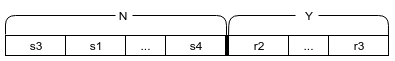
\includegraphics[scale=0.7]{WusnEncode.png}
    \captionof{figure}{Ví dụ mã hóa 1 cá thể}
\end{center}

Giải mã cá thể được thực hiện như sau: mỗi dãy $N/Y$ cảm biến liên tiếp sẽ được gắn với relay có thứ tự tương ứng.

\begin{center}
    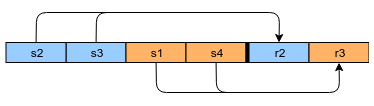
\includegraphics[scale=0.7]{WusnDecode.png}
    \captionof{figure}{Ví dụ giải mã 1 cá thể}
\end{center}

Bằng cách mã hóa này, ta có thể sử dụng các toán tử di truyền đã được nghiên cứu dành cho dãy số và dãy hoán vị.

\section{Sinh quần thể ban đầu}
Nhóm đề xuất 1 heuristic ngẫu nhiên cho việc sinh quần thể ban đầu. 

Xét không gian 2 chiều chứa tất cả các cảm biến. Sử dụng giải thuật phân cụm k-means, chia các cảm biến thành $Y$ cụm có tâm $r^*_y$. Với mỗi cụm, chọn 1 relay chưa được chọn có mất mát đường truyền đối với $r^*_y$ nhỏ nhất.

Một vấn đề đặt ra là k-means không kiểm soát được số lượng phần tử trong 1 cụm, làm cho các relay có thể vi phạm điều kiện cân bằng. Nhóm giải quyết vấn đề này bằng cách đơn giản là đặt các cảm biến và relay của mỗi cụm liên tiếp nhau trong quá trình mã hóa. Điều này đồng nghĩa với việc 1 số cảm biến sẽ bị chuyển từ cụm này sang cụm khác. Chất lượng lời giải có thể bị suy giảm, tuy nhiên điều này là chấp nhận được đối với quần thể ban đầu trong khi không ảnh hưởng nhiều đến tốc độ của toàn bộ thuật toán.

Dễ thấy rằng lời giải thu được luôn là chấp nhận được. Do khởi tạo của k-means là ngẫu nhiên, thuật toán trên sẽ cho các kết quả khác nhau trong mỗi lần chạy. Ta chạy thuật toán nhiều lần để sinh các cá thể khác nhau cho quần thể ban đầu.

\section{Lai ghép}
Do các cá thể gồm 2 phần, việc áp dụng các toán tử di truyền cũng cần được áp dụng trên từng phần của cá thể.

Đối với phần sensor, ta nhận thấy đây là 1 hoán vị tương tự mã hóa được dùng trong bài toán TSP. Nhóm sử dụng 1 toán tử phổ biến cho TSP là PMX (Partially Mapped Crossover).

Với phần relay, nhóm sử dụng lai ghép 2 điểm cắt, sau đó thay thế bất kì relay nào trùng nhau bằng 1 relay ngẫu nhiên nằm ngoài dãy.

\section{Đột biến}
Đối với phần sensor, phép đột biến đơn giản là hoán đổi vị trí của 2 cảm biến ngẫu nhiên.

Đối với phần relay, phép đột biến được thực hiện như sau. Chọn 1 relay ngẫu nhiên trong tập tất cả các relay. Nếu relay này không nằm trong cá thể, thay thế 1 relay ngẫu nhiên trong cá thể bằng relay này. Ngược lại, đổi chỗ của relay này với 1 relay ngẫu nhiên khác.

\section{Lựa chọn cá thể}
Hàm đánh gía các cá thể là hàm trả về giá trị mất mát đường truyền lớn nhất của lời giải tương ứng.

Các cá thể được lựa chọn theo chiến thuật tournament. Chọn ngẫu nhiên 1 tập con của quần thể, sau đó chọn $n$ cá thể tốt nhất trong tập con được chọn.

\chapter{Kêt quả thực nghiệm}
\section{Dữ liệu thử nghiệm}
Nhóm thực hiện sinh ngẫu nhiên 2 tập dữ liệu để thử nghiệm và đánh giá mô hình.
\begin{itemize}
    \item Tập Full: 10 đầu vào có kích cỡ vùng 1000x1000, N = 200, M = 200, Y = 20. Tập dữ liệu này được xây dựng với cấu hình giống với \cite{YuanWusn}.
    \item Tập Small: 10 đầu vào có kích cỡ vùng 200x200, N = 40, M = 40, Y = 4. Tập này có kích cỡ nhỏ hơn và được dùng chủ yếu để kiểm thử. Do giới hạn về thời gian thử nghiệm, nhóm sẽ chỉ báo cáo kết quả trên tập này.
\end{itemize}

\section{Cài đặt}
Nhóm thực hiện cài đặt lại các thuật toán heuristic trong \cite{YuanWusn} và thuật toán được đề xuất.

Các thuật toán được cài đặt bằng Python. Giải thuật di truyền được cài đặt dựa trên thư viện \textit{deap}.

\section{Kết quả}
Kết quả thực nghiệm được cho trong bảng sau. Do các thuật toán heuristic là tất định, nhóm chỉ thực hiện 1 lần chạy cho các thuật toán này. Với thuật toán được đề xuất, nhóm lấy kết quả sau 20 lần chạy với mỗi dữ liệu.

Giải thuật di truyền được chạy tối đa 10,000 thế hệ và dừng sớm nếu không có cải thiện sau 40 thế hệ. Quần thể có kích cỡ 70. Xác suất lai ghép bằng 80\%, xác suất đột biến bằng 5\%. Tập con cho lựa chọn tournament có kích cỡ bằng 0.8 kích cỡ quần thể.

\begin{table}[]
\centering
\begin{tabular}{|c|c|c|c|c|c|c|c|c|}
\hline
\diagbox[width=6em]{Test}{Thuật\\toán} & \multicolumn{2}{c|}{\textbf{LU1/LB3}} & \multicolumn{2}{c|}{\textbf{LU2/LB3}} & \multicolumn{3}{c|}{\textbf{GA w/ Clustering}} \\ \hline
\multicolumn{1}{|l|}{}          & t (ms)         & Loss        & t (ms)           & Loss           & Avg. t (ms)  & Avg. Loss  & Min Loss \\ \hline
\textbf{1} & 62.64 & 256.73 & 2321.90 & 271.43 & 179013.99 & 248.00 & 240.82 \\ \hline
\textbf{2} & 47.36 & 255.43 & 2292.88 & 268.88 & 187870.14 & 248.81 & 239.20 \\ \hline
\textbf{3} & 51.12 & 256.90 & 2306.35 & 266.26 & 180623.50 & 249.18 & 242.89 \\ \hline
\textbf{4} & 49.88 & 251.14 & 2434.52 & 273.09 & 199641.77 & 249.95 & 241.36 \\ \hline
\textbf{5} & 47.61 & 257.40 & 2366.93 & 280.79 & 214119.68 & 247.97 & 242.99 \\ \hline
\textbf{6} & 50.02 & 261.66 & 2384.48 & 262.81 & 206661.67 & 252.89 & 243.13 \\ \hline
\textbf{7} & 94.37 & 257.11 & 2367.25 & 274.89 & 222644.89 & 251.03 & 247.45 \\ \hline
\textbf{8} & 52.71 & 247.77 & 2393.78 & 277.49 & 200350.64 & 250.34 & 245.50 \\ \hline
\textbf{9} & 49.10 & 258.66 & 2903.16 & 276.62 & 195602.57 & 243.20 & 238.84 \\ \hline
\textbf{10} & 51.29 & 259.50 & 2897.00 & 272.32 & 196454.75 & 248.76 & 241.63 \\ \hline
\end{tabular}
\caption{Kết quả thực nghiệm trên bộ dữ liệu Small}
\end{table}

\section{Kết luận}
Có thể nhận thấy việc sử dụng giải thuật đề xuất đa phần cho kết quả tốt hơn so với sử dụng heuristic. Tuy nhiên, ta trả giá bằng thời gian chạy lâu hơn.

Hướng phát triển của nhóm bao gồm:
\begin{itemize}
    \item Thử nghiệm với các toán tử di truyền và đột biến khác.
    \item Cải thiện thời gian chạy của thuật toán.
    \item Kết hợp các heuristic vào quá trình khởi tạo.
\end{itemize}

\begin{thebibliography}{9}
\bibitem{YuanWusn} Bo Yuan, Huanhuan Chen, Xin Yao, \textit{Optimal Relay Placement for Lifetime Maximization in Wireless Underground Sensor Networks}, Information Sciences, 2017.

\end{thebibliography}
\end{document}
